\subsection{Rare Group Trajectories}\label{apdx:rare_macrostates}

\begin{figure}[h]
    \centering
    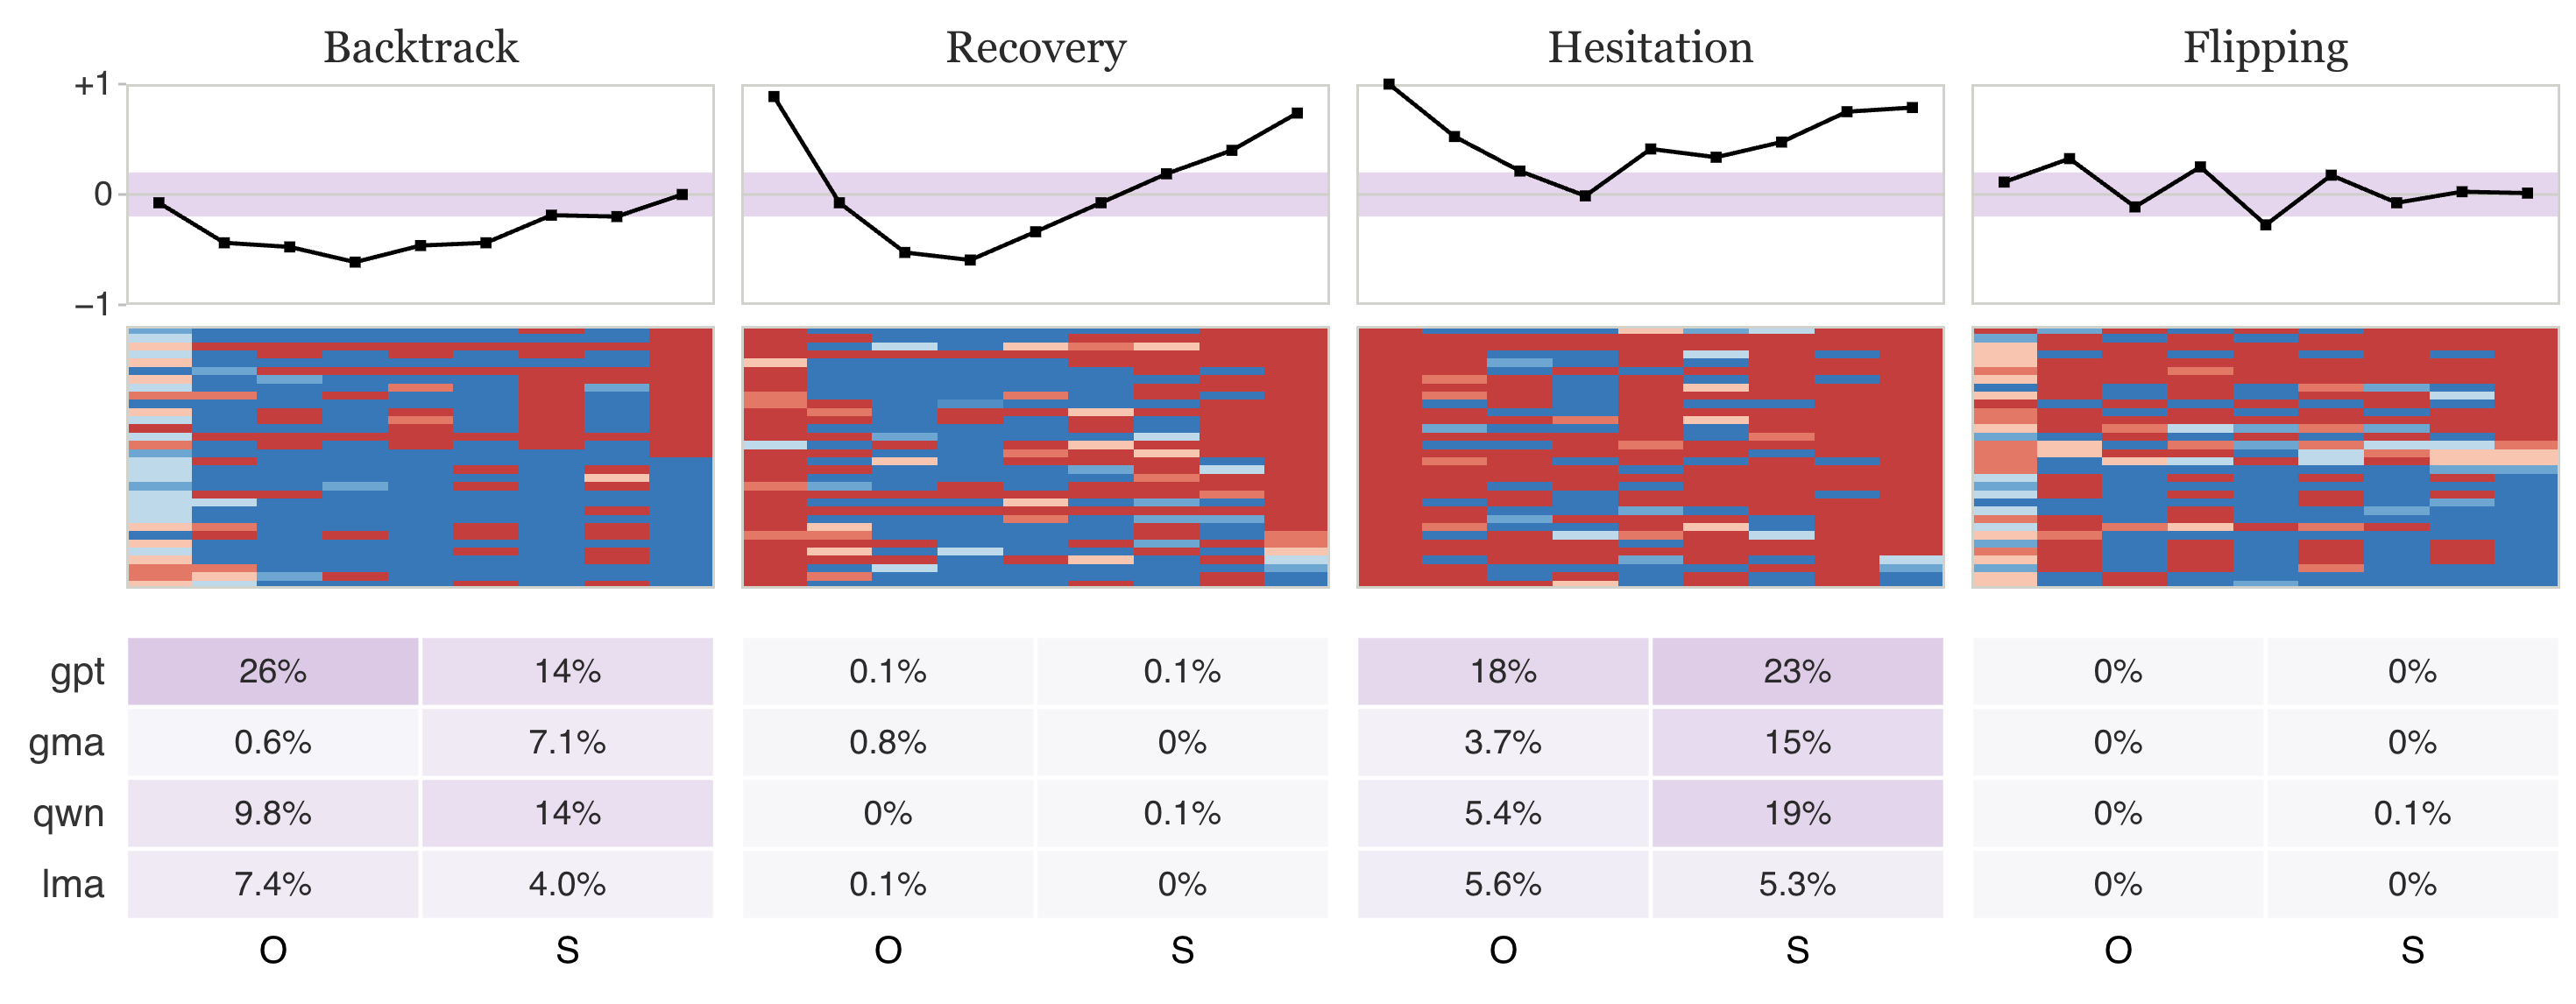
\includegraphics[width=0.99\textwidth]{main/Figures/apx_06_rare_macrostates.png}
\caption{\textit{Rare and non-monotone group trajectories.}
Groups whose net opinion \emph{reverses
direction} mid-run, which a first-vs-last-round classification cannot distinguish. Same setup as
Figure ~\ref{fig:macrostates}. A \emph{strong majority} denotes a round with absolute net opinion $|n(t)| \geq 0.5$, which is beyond the
split band $ \le \delta = 0.2$.}
\label{fig:rare_macrostates}
\end{figure} 

\emph{Backtrack}: A split community (absolute net opinion in $\pm 0.2$ split band) first develops a strong majority (absolute net opinion $\geq 0.5$) before relaxing back toward a split. \emph{Recovery}: A strong majority (absolute net opinion $\geq 0.5$) reverses to the opposite side before returning to its original position. \emph{Hesitation}: A strong majority weakens almost to a split, then re-consolidates on the same side. \emph{Flipping}: The majority repeatedly changes sides during the simulation.

